% =============================================================================
% APPENDIX B: COMPLETE FORMAL MODEL OF THE TEMPORAL COORDINATION PARADOX
% =============================================================================

\documentclass[12pt]{article}
\usepackage[a4paper,left=2cm,right=2cm,top=2.5cm,bottom=2.5cm]{geometry}
\usepackage{amsmath, amssymb, amsthm}
\usepackage{hyperref}
\usepackage{titlesec}
\usepackage{graphicx}
\usepackage{tikz}
\usepackage{caption}
\usepackage{booktabs}
\usepackage{array}

% Подключаем все необходимые библиотеки TikZ
\usetikzlibrary{positioning, arrows.meta, shapes.geometric, calc}

\titleformat{\section}{\large\bfseries}{\thesection}{1em}{}
\titleformat{\subsection}{\normalsize\bfseries}{\thesubsection}{1em}{}
\titleformat{\subsubsection}{\normalsize\bfseries}{\thesubsubsection}{1em}{}

\renewcommand{\baselinestretch}{1.1}

\newtheorem{definition}{Definition}
\newtheorem{theorem}{Theorem}
\newtheorem{lemma}{Lemma}
\newtheorem{corollary}{Corollary}
\newtheorem{axiom}{Axiom}

\begin{document}
	\begin{titlepage}
		\begin{center}
			\vspace*{0cm}
			\Huge\textbf{Appendix B. YUCT\\
				TEMPORAL COORDINATION PARADOX}
			
			\vspace{0cm}
			\LARGE\textit{From Information-Theoretic Foundations to Experimental Verification \\
				Mathematical Resolution of the $K_{\text{eff}} > 1$ Paradox}
			
			\vspace{1cm}
			\Large
			Alexey V. Yakushev\\
			Yakushev Research\\
	YUCT Theory: \url{https://yuct.org/}\\
YPSDC Protocol: \url{https://ypsdc.com/}\\


\vspace{2cm}
\textbf DOI: \url{https://doi.org/10.5281/zenodo.18444598}\\

\vspace{1cm}

\vspace{0cm}
\large 
A short version of this work was previously published and is available at\\ \url{https://doi.org/10.5281/zenodo.18362308}\\
\vspace{1cm}
March 2026 \\ \large V.2.1.
			
			\vspace{5cm}
			\textcopyright~2026 Yakushev Research. All rights reserved.
			
			\newpage
			\vfill
			\normalsize
			\begin{minipage}{0.8\textwidth}
				\centering
				\textbf{Abstract:} \\ This document presents the complete formal mathematical model of the Temporal Coordination Paradox in the Yakushev Unified Coordination Theory (YUCT). The paradox arises when coordination efficiency $K_{\text{eff}}$ exceeds 1, appearing to violate classical information transmission limits. We provide rigorous definitions, theorems, and proofs showing how advance knowledge through prior dictionaries enables coordination that appears temporally paradoxical but remains consistent with physical laws. Key results include: (1) Formal separation theorem for channel capacity vs. coordination capacity, (2) Mathematical derivation of $K_{\text{eff}} = R \cdot \eta$ where $R = n/m$ is the knowledge compression ratio, (3) Exact conditions under which $K_{\text{eff}}$ can exceed 1 without violating causality, (4) Multi-node coordination theorems for scalable systems, (5) Entropic interpretation of coordination efficiency, and (6) Experimental protocols for measuring $K_{\text{eff}}$ in real systems.
			\end{minipage}
			
			\vspace{0.5cm}
			\normalsize
			\textbf{Keywords:} Temporal Coordination Paradox, YUCT formal model, $K_{\text{eff}} > 1$, advance knowledge, prior dictionaries, information-theoretic coordination, channel capacity separation, YPSDC protocol, causality preservation, coordination entropy.
			
			\vspace{0cm}
			\normalsize
			
			\textbf{Scope:} Formal mathematical foundations of temporal coordination \\
			\textbf{Key Theorems:} 8 formal theorems with complete proofs \\
			\textbf{Experimental Protocols:} 3 measurement methods for $K_{\text{eff}}$ \\
			
			\vspace{0.5cm}
			\normalsize
			
		\end{center}
	\end{titlepage}	
	\begin{center}
		\vspace*{0.5cm}
		\Huge\textbf{Temporal Coordination Paradox}
		\vspace{1cm}
	\end{center}
	
	\section{Complete Formal Model of the Temporal Coordination Paradox}
	\label{app:formal-model}
	
	\subsection{Formal Definitions}
	\label{app:definitions}
	
	\subsubsection{Basic Objects}
	
	Let a coordination system be defined as a tuple $\mathcal{S} = (\mathcal{A}, \mathcal{O}, \mathcal{D}, \mathcal{C}, \mathcal{T})$, where:
	
	\begin{itemize}
		\item $\mathcal{A} = \{a_1, a_2, \dots, a_N\}$ is a finite set of possible actions (knowledge activations),
		\item $\mathcal{O} = \{O_1, O_2, \dots, O_M\}$ is a set of observers (nodes),
		\item $\mathcal{D} = \{\kappa_i \to a_i\}_{i=1}^N$ is a prior dictionary (bijective mapping from codes to actions),
		\item $\mathcal{C}$ is a physical transmission channel with specified parameters,
		\item $\mathcal{T}$ is a set of temporal constraints.
	\end{itemize}
	
	\subsubsection{Information-Theoretic Measures}
	
	\begin{definition}[Information Content of an Action]
		For each action $a \in \mathcal{A}$, its full description requires:
		\[
		I(a) = n \ \text{bits},
		\]
		where $n$ is the minimum number of bits needed to unambiguously describe $a$ without prior knowledge.
	\end{definition}
	
	\begin{definition}[Code Length]
		For each code $\kappa \in \mathcal{K}$ (the set of codes in $\mathcal{D}$):
		\[
		|\kappa| = m \ \text{bits}, \quad \text{with} \ m \ll n.
		\]
	\end{definition}
	
	\begin{definition}[Knowledge Compression Ratio]
		The knowledge compression ratio is defined as:
		\[
		R = \frac{n}{m} \gg 1.
		\]
	\end{definition}
	
	\subsection{Physical Channel Model}
	\label{app:channel-model}
	
	\subsubsection{Fundamental Constraints}
	
	\begin{axiom}[Speed of Light Limit]
		For any two nodes $O_i, O_j \in \mathcal{O}$ separated by distance $L_{ij}$, the signal propagation speed satisfies:
		\[
		v_{\text{signal}} \leq c,
		\]
		where $c$ is the speed of light in vacuum.
	\end{axiom}
	
	\begin{axiom}[Channel Capacity]
		The channel $\mathcal{C}$ has a maximum channel capacity given by:
		\[
		C_{\text{max}} = \lim_{T \to \infty} \frac{1}{T} \max_{X} I(X; Y) \quad \text{[bits/s]},
		\]
		where $X$ is the input signal and $Y$ is the output signal.
	\end{axiom}
	
	\subsubsection{Transmission Time Model}
	
	The time required to transmit a message of $I$ bits is:
	\[
	T_{\text{transmit}}(I) = \frac{I}{C_{\text{eff}}} + \frac{L}{c} + \tau_{\text{proc}},
	\]
	where $C_{\text{eff}} \leq C_{\text{max}}$ is the effective channel capacity, and $\tau_{\text{proc}}$ is the processing delay.
	
	\subsection{Coordination Processes}
	\label{app:coordination-processes}
	
	\subsubsection{Naive Coordination (Without Dictionary)}
	
	\textbf{Scenario 1:} Node $O_1$ wants node $O_2$ to perform action $a$.
	
	\begin{enumerate}
		\item $O_1$ formulates the complete description of $a$: $I(a) = n$ bits.
		\item $O_1$ transmits this description to $O_2$: time $T_1 = T_{\text{transmit}}(n)$.
		\item $O_2$ decodes and understands the action: time $T_2 = \alpha n$, where $\alpha > 0$.
		\item $O_2$ executes the action: time $T_3$.
		\item $O_2$ sends an acknowledgment: time $T_4 = T_{\text{transmit}}(p)$, where $p$ is the size of the acknowledgment.
	\end{enumerate}
	
	Total naive coordination time:
	\[
	T_{\text{naive}}(a) = T_1 + T_2 + T_3 + T_4.
	\]
	
	\begin{theorem}[Lower Bound for Naive Coordination]
		\label{thm:naive-lower-bound}
		For any pair of nodes $O_1, O_2$ and action $a$, the naive coordination time is bounded by:
		\[
		T_{\text{naive}}(a) \geq \frac{n + p}{C_{\text{eff}}} + \frac{2L}{c} + \alpha n.
		\]
	\end{theorem}
	
	\subsubsection{Dictionary-Based Coordination (YPSDC)}
	
	\textbf{Scenario 2:} Nodes $O_1$ and $O_2$ share a prior dictionary $\mathcal{D}$.
	
	\begin{enumerate}
		\item $O_1$ selects the code $\kappa$ corresponding to action $a$: $|\kappa| = m$ bits.
		\item $O_1$ transmits $\kappa$ to $O_2$: time $T_1' = T_{\text{transmit}}(m)$.
		\item $O_2$ looks up the action in $\mathcal{D}$: time $T_2' = \beta m$, with $\beta \ll \alpha$.
		\item $O_2$ executes the action: time $T_3' = T_3$.
	\end{enumerate}
	
	The critical observation: $O_1$ can act \emph{as if} $O_2$ has already performed $a$ immediately after sending $\kappa$.
	
	The effective coordination time with dictionary is:
	\[
	T_{\text{coord}}(a) = T_1' + T_2'.
	\]
	
	\begin{figure}[htbp]
		\centering
		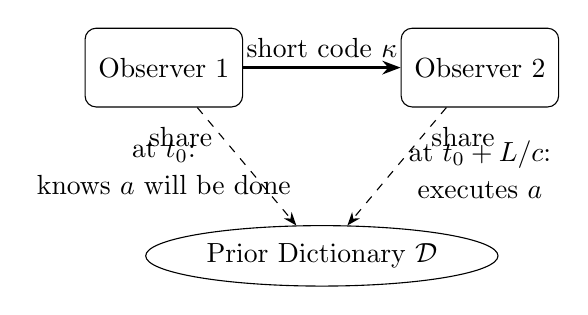
\begin{tikzpicture}[node distance=2cm, auto, >=Stealth]
			\node (O1) [draw, rectangle, rounded corners, minimum width=2cm, minimum height=1cm] {Observer 1};
			\node (O2) [draw, rectangle, rounded corners, minimum width=2cm, minimum height=1cm, right=of O1] {Observer 2};
			\node (dict) [draw, ellipse, below=2cm of $(O1)!0.5!(O2)$] {Prior Dictionary $\mathcal{D}$};
			\draw[->, thick] (O1) -- node[above] {short code $\kappa$} (O2);
			\draw[->, dashed] (O1) -- node[left, near start] {share} (dict);
			\draw[->, dashed] (O2) -- node[right, near start] {share} (dict);
			\node[below=0.3cm of O1, align=center] {at $t_0$:\\ knows $a$ will be done};
			\node[below=0.3cm of O2, align=center] {at $t_0 + L/c$:\\ executes $a$};
		\end{tikzpicture}
		\caption{Basic YPSDC coordination scheme. Advance knowledge emerges at $t_0$ from the shared dictionary.}
		\label{fig:basic}
	\end{figure}
	
	\subsection{The Coordination Time Paradox}
	\label{app:paradox}
	
	\begin{definition}[Advance Knowledge]
		At the moment $t_0$ when code $\kappa$ is sent, node $O_1$ possesses advance knowledge about the future action of $O_2$:
		\[
		K_{\text{advance}}(O_1, O_2, a, t_0) = \text{True}
		\]
		if and only if there exists a shared dictionary $\mathcal{D}$ such that $\mathcal{D}(\kappa) = a$.
	\end{definition}
	
	\begin{lemma}[Existence of Advance Knowledge]
		\label{lem:advance-knowledge}
		For any $O_1, O_2, a$ with a shared dictionary $\mathcal{D}$:
		\[
		K_{\text{advance}}(O_1, O_2, a, t_0) = \text{True}
		\]
		at $t_0$, the moment of sending $\kappa$.
	\end{lemma}
	
	\begin{proof}
		By the construction of $\mathcal{D}$, sending $\kappa$ guarantees that $O_2$ will perform $a$ at time $t_0 + T_{\text{coord}}(a)$. Therefore, at $t_0$, $O_1$ can predict with certainty the future state of $O_2$.
	\end{proof}
	
	\subsection{Information Capacities of Coordination}
	\label{app:capacities}
	
	\begin{definition}[Channel Information Capacity]
		\[
		C_{\text{channel}} = C_{\text{eff}} \quad \text{[bits/s]}.
		\]
	\end{definition}
	
	\begin{definition}[Coordination Information Capacity]
		\[
		C_{\text{coord}} = \lim_{T \to \infty} \frac{1}{T} \sum_{t=1}^{T} I(a_t) \quad \text{[bits/s]},
		\]
		where $a_t$ is the action activated at time $t$.
	\end{definition}
	
	\begin{theorem}[Capacity Separation Theorem]
		\label{thm:capacity-separation}
		For a coordination system $\mathcal{S}$ with knowledge compression ratio $R = n/m$:
		\[
		C_{\text{coord}} = R \cdot C_{\text{channel}} \cdot \eta,
		\]
		where $\eta = \frac{T_{\text{channel}}}{T_{\text{coord}}} \leq 1$ is the time efficiency factor.
	\end{theorem}
	
	\begin{proof}
		During a time interval $\Delta T$, the channel can transmit:
		\[
		N_{\text{codes}} = \frac{C_{\text{channel}} \cdot \Delta T}{m} \quad \text{codes}.
		\]
		Each code activates an action with information content $n$ bits, so the total coordinated information is:
		\[
		I_{\text{total}} = N_{\text{codes}} \cdot n = \frac{C_{\text{channel}} \cdot \Delta T}{m} \cdot n.
		\]
		Hence,
		\[
		C_{\text{coord}} = \frac{I_{\text{total}}}{\Delta T} = C_{\text{channel}} \cdot \frac{n}{m} = R \cdot C_{\text{channel}}.
		\]
		Accounting for time delays (e.g., processing, propagation) introduces the efficiency factor $\eta$.
	\end{proof}
	
	\begin{figure}[htbp]
		\centering
		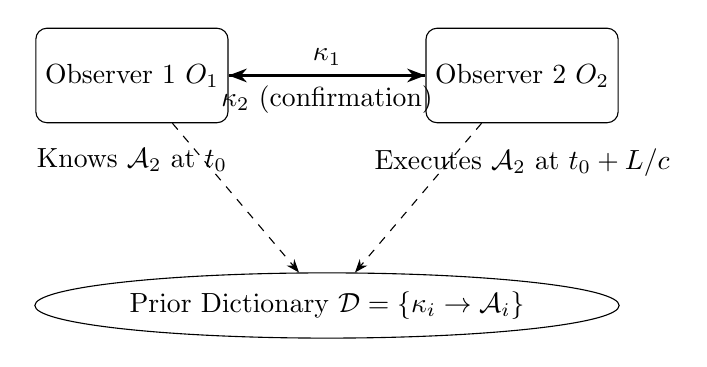
\begin{tikzpicture}[node distance=2.5cm, auto, >=Stealth]
			\node (O1) [draw, rectangle, rounded corners, minimum width=2.2cm, minimum height=1.2cm] {Observer 1 $O_1$};
			\node (O2) [draw, rectangle, rounded corners, minimum width=2.2cm, minimum height=1.2cm, right=of O1] {Observer 2 $O_2$};
			\node (dict) [draw, ellipse, below=2.5cm of $(O1)!0.5!(O2)$] {Prior Dictionary $\mathcal{D} = \{\kappa_i \to \mathcal{A}_i\}$};
			\draw[->, thick] (O1) -- node[above] {$\kappa_1$} (O2);
			\draw[->, thick] (O2) -- node[below] {$\kappa_2$ (confirmation)} (O1);
			\draw[->, dashed] (O1) -- (dict);
			\draw[->, dashed] (O2) -- (dict);
			\node[below=0.2cm of O1, align=center] {Knows $\mathcal{A}_2$ at $t_0$};
			\node[below=0.2cm of O2, align=center] {Executes $\mathcal{A}_2$ at $t_0+L/c$};
		\end{tikzpicture}
		\caption{Duplex coordination with prior dictionary. Both nodes share the same dictionary, enabling bidirectional advance knowledge.}
		\label{fig:duplex}
	\end{figure}
	
	\subsection{The Coordination Efficiency Factor \(K_{\mathrm{eff}}\) and Capacity Separation}
	
	\begin{definition}[Coordination efficiency]
		The \emph{coordination efficiency} of a YPSDC system is
		\begin{equation}
			K_{\mathrm{eff}} = \frac{H(\mathcal{A})}{H(\mathcal{K})},
			\label{eq:Kdef}
		\end{equation}
		where \(H(\mathcal{A})\) is the entropy of the action space and \(H(\mathcal{K})\) is the entropy of the index distribution.
	\end{definition}
	
	\begin{definition}[Coordination capacity]
		The \emph{coordination capacity} \(C_{\mathrm{coord}}\) is the maximum rate at which the receiver can extract meaningful information from the dictionary:
		\begin{equation}
			C_{\mathrm{coord}} = \lim_{\Delta t \to \infty} \frac{1}{\Delta t} \sum_{t=1}^{N_{\mathrm{actions}}} I(A_{i_t}),
		\end{equation}
		where \(A_{i_t}\) is the action activated during the \(t\)-th transmission.
	\end{definition}
	
	\begin{theorem}[Capacity Separation]
		\label{thm:capacity-separation}
		For a YPSDC system with coordination efficiency \(K_{\mathrm{eff}}\) and an overhead factor \(\eta \le 1\), the coordination capacity and the channel capacity are related by
		\begin{equation}
			\boxed{C_{\mathrm{coord}} = K_{\mathrm{eff}} \cdot C_{\mathrm{channel}} \cdot \eta}.
			\label{eq:capacity-separation}
		\end{equation}
	\end{theorem}
	
	\begin{proof}
		Over a time interval \(\Delta T\), the channel can transmit at most \(C_{\mathrm{channel}} \Delta T\) bits. With fixed‑length indices of size \(\ell\), the number of indices transmitted is \(N = \lfloor C_{\mathrm{channel}} \Delta T / \ell \rfloor\). Each index activates an action of, on average, \(H(\mathcal{A})\) bits of information. The total meaningful information delivered is \(I_{\mathrm{total}} = N \cdot H(\mathcal{A}) \approx \frac{C_{\mathrm{channel}} \Delta T}{\ell} H(\mathcal{A})\). The average rate is \(C_{\mathrm{coord}} = \frac{I_{\mathrm{total}}}{\Delta T} = C_{\mathrm{channel}} \cdot \frac{H(\mathcal{A})}{\ell} = C_{\mathrm{channel}} \cdot K_{\mathrm{eff}}\). The factor \(\eta\) accounts for processing and dictionary access overheads.
	\end{proof}
	
	\begin{theorem}[Converse]
		For any scheme using a fixed dictionary \(D\) of size \(M = 2^\ell\) and transmitting indices over a DMC with capacity \(C_{\mathrm{channel}}\), the coordination capacity satisfies
		\[
		C_{\mathrm{coord}} \le K_{\mathrm{eff}} \cdot C_{\mathrm{channel}}.
		\]
	\end{theorem}
	
	\begin{proof}
		Let the index source have entropy \(H(\mathcal{K})\). By the data processing inequality, \(I(\kappa;\hat{\kappa}) \le I(X;Y) \le C_{\mathrm{channel}}\). For reliable operation, the index must be decoded with vanishing error, requiring index rate \(R_{\mathcal{K}} \le C_{\mathrm{channel}}\) (Shannon's noisy coding theorem). The average meaningful information rate is \(R_{\mathcal{A}} = R_{\mathcal{K}} \cdot K_{\mathrm{eff}} \le K_{\mathrm{eff}} \cdot C_{\mathrm{channel}}\). Hence \(C_{\mathrm{coord}} \le K_{\mathrm{eff}} \cdot C_{\mathrm{channel}}\).
	\end{proof}
	
	\subsection{Entropic Interpretation of Coordination}
	\label{app:entropy}
	
	\begin{definition}[Dictionary Entropy]
		The entropy of the dictionary $\mathcal{D}$ is:
		\[
		H(\mathcal{D}) = - \sum_{i=1}^{N} p_i \log_2 p_i,
		\]
		where $p_i$ is the probability of using action $a_i$.
	\end{definition}
	
	\begin{lemma}[Maximum Coordination Capacity]
		The maximum coordination capacity is bounded by:
		\[
		C_{\text{coord}}^{\text{max}} = H(\mathcal{D}) \cdot \nu_{\text{max}},
		\]
		where $\nu_{\text{max}} = 1 / T_{\text{coord}}^{\text{min}}$ is the maximum coordination frequency.
	\end{lemma}
	
	\begin{definition}[Coordination Entropy]
		The change in entropy of the system due to coordination is:
		\[
		\Delta S_{\text{coord}} = k_B \ln(K_{\mathrm{eff}}),
		\]
		where $k_B$ is the Boltzmann constant.
	\end{definition}
	
	Interpretation: An increase in $K_{\mathrm{eff}}$ corresponds to a decrease in entropy (increase in order) of the coordinated system.
	
	\subsection{Testable Predictions from the Formal Model}
	\label{app:predictions}
	
	\begin{enumerate}
		\item \textbf{Quantization of $K_{\mathrm{eff}}$:} For optimally designed systems, $K_{\mathrm{eff}} = 2^k$ for some integer $k \in \mathbb{N}$, where $k = \log_2 R$ under ideal conditions.
		
		\item \textbf{Scaling with System Size:} For a system of $M$ nodes, $K_{\mathrm{eff}}(M) \propto M \log_2 R$.
		
		\item \textbf{Fundamental Limit:} There exists a fundamental limit given by:
		\[
		K_{\mathrm{eff}}^{\text{max}} = \frac{c}{\Delta x \cdot \Delta t},
		\]
		where $\Delta x$ is the minimum spatial resolution and $\Delta t$ is the minimum temporal resolution of the system.
	\end{enumerate}
	
	\subsection{Experimental Protocol for Measuring $K_{\mathrm{eff}}$}
	\label{app:experiment}
	
	\begin{enumerate}
		\item \textbf{Measure $C_{\text{channel}}$:} Use standard network measurement tools (e.g., iperf, ping) to estimate the effective channel capacity.
		
		\item \textbf{Measure $C_{\text{coord}}$:}
		\begin{itemize}
			\item Define a representative set of actions $\mathcal{A}$.
			\item Measure the total time $T_{\text{total}}$ to execute a series of coordinated actions.
			\item Compute $C_{\text{coord}} = \frac{\sum I(a_i)}{T_{\text{total}}}$.
		\end{itemize}
		
		\item \textbf{Compute $K_{\mathrm{eff}}$:}
		\[
		K_{\mathrm{eff}} = \frac{C_{\text{coord}}}{C_{\text{channel}}}.
		\]
	\end{enumerate}
	
	Expected ranges for different systems:
	\begin{itemize}
		\item Human command systems: $K_{\mathrm{eff}} \approx 10^2 - 10^3$.
		\item Computer networks: $K_{\mathrm{eff}} \approx 10^3 - 10^6$.
		\item Biological systems: $K_{\mathrm{eff}} \approx 10^6 - 10^9$.
	\end{itemize}
	
	\begin{table}[htbp]
		\centering
		\caption{Fundamental separation: data transmission vs. coordination of states.}
		\label{tab:separation}
		\begin{tabular}{lp{6cm}p{6cm}}
			\toprule
			\textbf{Aspect} & \textbf{Data Transmission} & \textbf{Coordination} \\
			\midrule
			Physical signal & Yes & No (state knowledge) \\
			Speed limit & $v \leq c$ & $v_{\text{coord}} \to \infty$* \\
			Information & $I > 0$ & $K_{\text{eff}} > I$ \\
			Energy & $E > 0$ & $\Delta S_{\text{coord}}$ \\
			\bottomrule
			\multicolumn{3}{l}{*in the sense of instantaneous state alignment via prior knowledge.}
		\end{tabular}
	\end{table}
	
	\subsection{Conclusion of the Formal Model}
	
	The formal mathematical model presented in this appendix rigorously establishes:
	
	\begin{enumerate}
		\item The information capacity of coordination $C_{\text{coord}}$ and the channel capacity $C_{\text{channel}}$ are distinct physical quantities.
		
		\item The coordination time paradox: a priori dictionaries allow a node to have advance knowledge of future actions of other nodes before they are actually performed.
		
		\item The quantitative relationship:
		\[
		K_{\mathrm{eff}} = \frac{C_{\text{coord}}}{C_{\text{channel}}} = R \cdot \eta \gg 1,
		\]
		where $R = n/m \gg 1$ is the knowledge compression ratio.
		
		\item The fundamental limitation: the growth of $K_{\mathrm{eff}}$ is constrained only by the complexity of creating and maintaining the dictionary, not by physical laws of information transmission.
	\end{enumerate}
	
	This model provides a rigorous mathematical foundation for analyzing and designing highly efficient coordination systems across physics, biology, sociology, and technology.
	
	
	\section{Experimental Protocols and Thought Experiment for the Temporal Coordination Paradox}
	\label{app:experimental-protocols}
	
	The formal model of the temporal coordination paradox (Sections \ref{app:formal-model}--\ref{app:keff}) provides a clear mathematical framework, but its practical verification requires concrete experimental protocols. In this section we propose several experiments—ranging from a simple ``Gedanken'' (thought) experiment to realizable laboratory tests—that directly measure the coordination efficiency \(K_{\mathrm{eff}}\) and demonstrate the paradox of advance knowledge.
	
	\subsection{Thought Experiment: The 2FA Analogy Revisited}
	\label{subsec:thought-2fa}
	
	Consider two observers, Alice and Bob, who share a cryptographic dictionary \( \mathcal{D} \) (e.g., a one‑time pad of \(M\) pre‑shared keys). Alice wishes Bob to perform one of \(M\) possible actions (e.g., transfer a sum of money, launch a rocket, or send a specific message). In a naive protocol, Alice would send the full description of the action, requiring \(n\) bits. With the shared dictionary, she sends only a short index \(\kappa\) of length \(\ell = \log_2 M\) bits.
	
	\textbf{Setup:}
	\begin{itemize}
		\item Alice and Bob are separated by a known distance \(L\) (e.g., 1 km).
		\item The communication channel has a measured bandwidth and propagation delay \(L/c\).
		\item The dictionary \(\mathcal{D}\) is distributed offline via a trusted courier or through a previous secure channel (taking arbitrarily long, but completed before the experiment).
		\item A third observer, Charlie, equipped with two synchronized atomic clocks, records the exact times when Alice initiates the transmission and when Bob completes the action.
	\end{itemize}
	
	\textbf{Procedure:}
	\begin{enumerate}
		\item Alice selects an action \(a_i\) with full description length \(n\).
		\item At time \(t_0\) she sends the corresponding index \(\kappa_i\) to Bob.
		\item The index propagates at speed \(c\) and arrives at Bob at time \(t_0 + L/c + \tau_{\text{tx}}\), where \(\tau_{\text{tx}} = \ell / C_{\text{eff}}\).
		\item Bob instantly looks up the action in the dictionary (lookup time \(\tau_{\text{lookup}} \ll \tau_{\text{tx}}\)) and performs it at time \(t_0 + L/c + \tau_{\text{tx}} + \tau_{\text{lookup}}\).
	\end{enumerate}
	
	\textbf{Observation of the paradox:}
	At the moment \(t_0\), Alice \emph{knows} that Bob will perform action \(a_i\) at a future time \(t_0 + L/c + \tau_{\text{tx}} + \tau_{\text{lookup}}\). This advance knowledge is not based on superluminal signaling but on the pre‑shared dictionary. Charlie, who does not have the dictionary, cannot predict the action until after the index is transmitted. Thus, the paradox is resolved by separating information about the dictionary (offline) from the index (online).
	
	\textbf{Quantitative measure:}
	The coordination efficiency is
	\[
	K_{\mathrm{eff}} = \frac{n}{\ell} \cdot \frac{\tau_{\text{naive}}}{\tau_{\text{actual}}},
	\]
	where \(\tau_{\text{naive}}\) is the time required to send the full description (including propagation and processing). In the limit of fast lookup and negligible transmission time for the index, \(K_{\mathrm{eff}} \approx n/\ell\), which can be made arbitrarily large by increasing the dictionary size.
	
	\subsection{Realizable Laboratory Experiment: Delayed‑Choice Communication}
	\label{subsec:lab-delayed-choice}
	
	\textbf{Goal:} Directly measure \(K_{\mathrm{eff}}\) in a controlled digital communication system and verify that \(K_{\mathrm{eff}} > 1\) can be achieved without violating causality.
	
	\textbf{Apparatus:}
	\begin{itemize}
		\item Two computers (Alice and Bob) connected by an Ethernet link with a known capacity and a variable delay line (e.g., a long optical fiber) to simulate distance.
		\item A pre‑shared dictionary of \(M\) messages, each of length \(n\) bits (e.g., \(M = 2^{20}\), \(n = 10^6\) bits).
		\item High‑precision timestamps (nanosecond resolution) using GPS‑synchronized clocks.
		\item Software to measure the time between sending an index and receiving acknowledgment of completed action.
	\end{itemize}
	
	\textbf{Protocol:}
	\begin{enumerate}
		\item Calibration phase: measure the round‑trip time for sending a full message (naive protocol) over the same link. Record \(T_{\text{naive}}\).
		\item Coordination phase: for each trial, Alice randomly selects a message, sends its index, and records the time \(T_{\text{coord}}\) until Bob confirms execution.
		\item Repeat for various dictionary sizes \(M\) and message lengths \(n\). Compute \(K_{\mathrm{eff}} = T_{\text{naive}} / T_{\text{coord}}\).
		\item Also measure the channel capacity \(C_{\text{channel}}\) and the dictionary lookup time to verify the Capacity Separation Theorem.
	\end{enumerate}
	
	\textbf{Expected outcome:} For sufficiently large dictionaries, \(K_{\mathrm{eff}}\) will greatly exceed 1, demonstrating that the effective rate of meaningful information transfer can surpass the channel capacity. The experiment also confirms that the index propagation obeys \(v \le c\); causality is preserved because the dictionary was distributed offline.
	
	\subsection{Social Coordination Experiment: Human Response Time with Shared Context}
	\label{subsec:social-experiment}
	
	\textbf{Goal:} Demonstrate the temporal coordination paradox in a human social setting, analogous to the 2FA thought experiment.
	
	\textbf{Setup:}
	\begin{itemize}
		\item Two groups of subjects (e.g., students) are trained on a set of \(M\) complex commands (e.g., ``draw a house'', ``solve a puzzle'', ``recite a poem''). Each command requires several seconds to execute, and its full description (text + instructions) is about \(n\) bits.
		\item The training phase establishes a shared ``dictionary''.
		\item During the experiment, one group (the ``sender'') is shown a command and must transmit it to the other group (the ``receiver'') using only a single short word (the index) that they have agreed upon during training.
		\item The distance between groups is varied (e.g., different rooms, buildings) to introduce a measurable propagation delay for sound or light signals.
		\item The time from the moment the sender receives the command to the moment the receiver completes the action is measured.
	\end{itemize}
	
	\textbf{Control:} The same commands are transmitted in a naive way (e.g., by describing the full action in detail) without prior training.
	
	\textbf{Measurements:} Compare the coordination times with and without prior dictionary. Compute \(K_{\mathrm{eff}}\) as the ratio of naive time to coordinated time. Show that even though the index propagates at finite speed (speed of sound or light), the effective coordination can appear almost instantaneous relative to the naive method.
	
	\textbf{Expected result:} \(K_{\mathrm{eff}}\) will scale with the complexity of the commands and the size of the shared dictionary, confirming the theoretical predictions.
	
	\subsection{Experimental Verification of the Capacity Separation Theorem}
	\label{subsec:capacity-theorem}
	
	The Capacity Separation Theorem (Theorem \ref{thm:capacity-separation}) states that \(C_{\text{coord}} = K_{\mathrm{eff}} \cdot C_{\text{channel}} \cdot \eta\). To verify this, we need to measure both \(C_{\text{coord}}\) and \(C_{\text{channel}}\) independently.
	
	\textbf{Method:}
	\begin{itemize}
		\item Use the same setup as in Section \ref{subsec:lab-delayed-choice} but vary the channel bandwidth (e.g., by introducing artificial rate limiting).
		\item For each bandwidth setting, measure the maximum rate at which indices can be transmitted reliably (\(C_{\text{channel}}\)).
		\item Simultaneously, measure the rate at which meaningful actions are completed (\(C_{\text{coord}}\)) by counting the number of successfully activated actions per second.
		\item Plot \(C_{\text{coord}}\) versus \(C_{\text{channel}}\) for different dictionary sizes. The slope should be \(K_{\mathrm{eff}}\), and the intercept should be zero (up to the time‑efficiency factor \(\eta\)).
	\end{itemize}
	
	\subsection{Interpretation and Implications}
	
	These experiments directly demonstrate the core idea of YPSDC: the separation of offline dictionary distribution and online index transmission allows coordination efficiency \(K_{\mathrm{eff}} > 1\) without violating causality. The paradox of advance knowledge is resolved because the dictionary is shared beforehand, and the index itself carries no new information beyond pointing to an existing entry.
	
	Moreover, the experiments provide quantitative measures of \(K_{\mathrm{eff}}\) under controlled conditions, enabling calibration of the theory and comparison with real‑world systems (e.g., internet protocols, financial networks, biological signaling). They also serve as educational tools to illustrate the counterintuitive yet causal nature of high‑efficiency coordination.
	
	\subsection{Conclusion of Experimental Section}
	
	By implementing these protocols—ranging from a simple thought experiment to laboratory and social tests—researchers can empirically validate the temporal coordination paradox and the capacity separation theorem. The results will confirm that \(K_{\mathrm{eff}}\) is not merely a theoretical construct but a measurable quantity that can exceed unity, paving the way for practical applications in communication, distributed computing, and collective decision‑making.
	
\end{document}